\documentclass[12pt,letterpaper,noanswers]{exam}
%\usepackage{color}
\usepackage[usenames,dvipsnames,svgnames,table]{xcolor}
\usepackage[margin=0.9in]{geometry}
\renewcommand{\familydefault}{\sfdefault}
\usepackage{multicol}
\pagestyle{head}
\usepackage{hyperref}
\definecolor{c07}{HTML}{BBFFBB}
\definecolor{c08}{HTML}{BBFFFF}
\definecolor{c09}{HTML}{BBDDFF}
\definecolor{c10}{HTML}{BBBBFF}
\definecolor{c11}{HTML}{DDBBFF}
\definecolor{c12}{HTML}{BBBBDD}
\newcommand{\mb}[1]{\underline{#1}}

\header{AM 22b Problem Set 07}{}{Due Thurs Apr 1 at 6pm}
\runningheadrule
\headrule
\usepackage{diagbox}
\usepackage{graphicx} % more modern
%\usepackage{subfigure} 
\usepackage{amsmath} 
\usepackage{amssymb} 
%\usepackage{gensymb} 
%\usepackage{natbib}
\usepackage{hyperref}
%\usepackage{enumitem}
%\setlength{\parindent}{0pt}
%\usepackage{setspace}
%\pagestyle{empty}  
%\newcommand{\Sc}[0]{
%{\color{BlueViolet}\S}
%}
\usepackage{tcolorbox}

\begin{document}
 \pdfpageheight 11in 
  \pdfpagewidth 8.5in

\begin{questions}
\question Log in to WeBWorK and complete the problems assigned there under pset07.


\question (line integrals)
\begin{parts}
\part The vector field $\mb F$ has $\Vert \mb F\Vert \leq 7$ everywhere.  Let $C$ be the circle of radius $1$ centered at the origin.  What is the largest value that $\displaystyle\oint_C \mb F\cdot d\mb r$ might have?  What is the most negative that it could potentially be?  What conditions lead to these values?
\part Give conditions on the constants $a$, $b$, and $c$ to ensure that the line integral $\displaystyle\int_C \mb F\cdot \mb T ds$ is positive, where $\mb F = a\mb i + b\mb j - \mb k$ and $C$ is the line segment from $(1,2,3)$ to $(1,2,c)$
\end{parts}

\question (more line integrals).
\begin{parts}
\part Explain why the following statement is true: whenever the circulation of a vector field around every closed curve is zero, the line integral along a curve with particular endpoints has a constant value independent of the path taken between the endpoints.

\emph{Provide a direct explanation, without assuming that circulation free vector fields are gradient fields.}
\part Explain why the \textbf{converse} to the statement is true:  whenever the line integral of a vector field depends only on the endpoints and not on the path between them, the circulation around every closed curve is zero.

\emph{Provide a direct explanation, without assuming that circulation free vector fields are gradient fields.}
\end{parts}


\item Use the Fundamental Theorem (of Line Integrals) to calculate $\int_C \vec F\cdot d\vec r$:
\begin{parts}
\part Compute $\int_C \left(\cos(xy)e^{\sin(xy)}(y\vec i + x\vec j)+\vec k\right)\cdot d\vec r$ where $C$ is the line from $(\pi,2,5)$ to $(0.5,\pi, 7)$.
\begin{solution}
To use the fundamental theorem, find $f$ such that $\vec F = \nabla f$, then find $f(end)-f(start)$ instead of computing the line integral.

We want $f$ such that $\vec F = f_x\vec i + f_y\vec j+f_z\vec k$ so we want $f_x = \cos(xy)e^{\sin(xy)}y$, $f_y = \cos(xy)e^{\sin(xy)}y$ and $f_z = 1$.

Using the $f_x$ information, we can learn about $f(x,y,z) \pm g(y,z)$ since $\frac{\partial}{\partial x}(f(x,y)\pm g(y)) = f_x$.

\[f(x,y,z)= \int \cos(xy)e^{\sin(xy)}y\ dx.\quad u = \sin(xy). \quad du = \cos(xy)y.\]
\[f(x,y,z)= \int e^udu = e^u = e^{\sin(xy)} + g(y,z).\]
Similarly, from the $f_y$ information we learn about $f(x,y,z) \pm h(x,z)$.
\[f(x,y,z)= \int \cos(xy)e^{\sin(xy)}y\ dy.\quad u = \sin(xy). \quad du = \cos(xy)x.\]
\[f(x,y,z) = \int e^udu = e^u = e^{\sin(xy)} + h(x,z).\]
Similarly, from the $f_z$ information we learn about $f(x,y,z) \pm q(x,y)$.
\[f(x,y,z)= \int 1\ dz = z + q(x,y).\]

Next we combine the information from these to find $f(x,y,z)$.  A term that depends on $x$ and $y$ will show up in the first two functions, but not the third.  One that depends on just $x$ will show up in the first, and one that depends on just $y$ will show up in the second.  Combining the information, we have one term that depends on $x$ and $y$.  It is repeated between the first two functions and not present in the third, just as it should be.  We also have a term that depends on $z$ and appears in just the third function.

We find $f(x,y,z) = e^{\sin(xy)}+z$ is a function such that $\vec F = \nabla f$.

The line integral is \[\int_C \vec F\cdot d\vec r  = f(0.5, \pi, 7) - f(\pi,2,5) = e^{\sin(\pi/2)}+7-(e^{\sin(2\pi)}+5) = 1+ 7-5 = 3\]
\end{solution}

\part Let $\vec F = 2x\vec i + 2y\vec j + 2z\vec k$.  Let $C$ be the line from the origin to $(1,4,9)$.  Find $\int_C \vec F\cdot d\vec r$.  Use the result to simplify the computation involved, and find \[\int_C \left((2x+y)\vec i + 2y\vec j + 2z\vec k\right)\cdot d\vec r.\]
\begin{solution}
We'll use the fundamental theorem for $\vec F$  It won't apply directly for $\vec F + y\vec i$, but it will help with that one, too.

For $\vec F$, we want $f_x = 2x, f_y = 2y, f_z = 2z$.  The three pieces of information we have lead to

$f(x,y,z) = x^2 + g(y,z)$,

$f(x,y,z) = y^2 + h(x,z)$,

$f(x,y,z) = z^2 + q(x,y)$.

Putting these together each of the three is giving us different information, so $f(x,y,z) = x^2+y^2+z^2 +c$ (where $c$ is some constant).

Using the fundamental theorem:
\[\int_C \vec F\cdot d\vec r = f(1,4,9)-f(0,0,0) = 1+16+81+c-c = 98.\]

Next we need to find
\[\int_C ((2x+y)\vec i + 2y\vec j + 2z\vec k)\cdot d\vec r.\]

This is \[\int_C (\vec F+y\vec i)\cdot d\vec r  =\int_C \vec F\cdot d\vec r + \int_C y\vec i \cdot d\vec r = 98+\int_C y\vec i\cdot d\vec r.\]

Parameterizing the curve, we care about the $\vec i$ component of $\frac{d\vec r}{dt}$ since that is the only direction where the vector field is nonzero.  We also care about $y(t)$ so that we can plug in to $\vec F$.  We can choose $x = t, y = 4t, z = 9t, 0\leq t\leq 1$ to parameterize our path.  So $\frac{dx}{dt} = 1$.  $\vec F(x(t),y(t),z(t)) = 4t\vec i$.

$\vec F \cdot \frac{d\vec r}{dt} = 4t$.  So \[\int_C y\vec i\cdot d\vec r = \int_0^1 4t\ dt = 2.\]

We have \[\int_C ((2x+y)\vec i + 2y\vec j + 2z\vec k)\cdot d\vec r = 98+2 = 100.\]
\end{solution}

\end{parts}

\question Consider the line integrals $\int_{C_i} \vec F\cdot d\vec r$ for $i = 1,2,3,4$ where $C_i$ is the path from $P_i$ to $Q_i$ shown in the figure below and where $\vec F = \nabla f$.  Level curves of $f$ are shown in the figure.  Include your reasoning for each of the following:

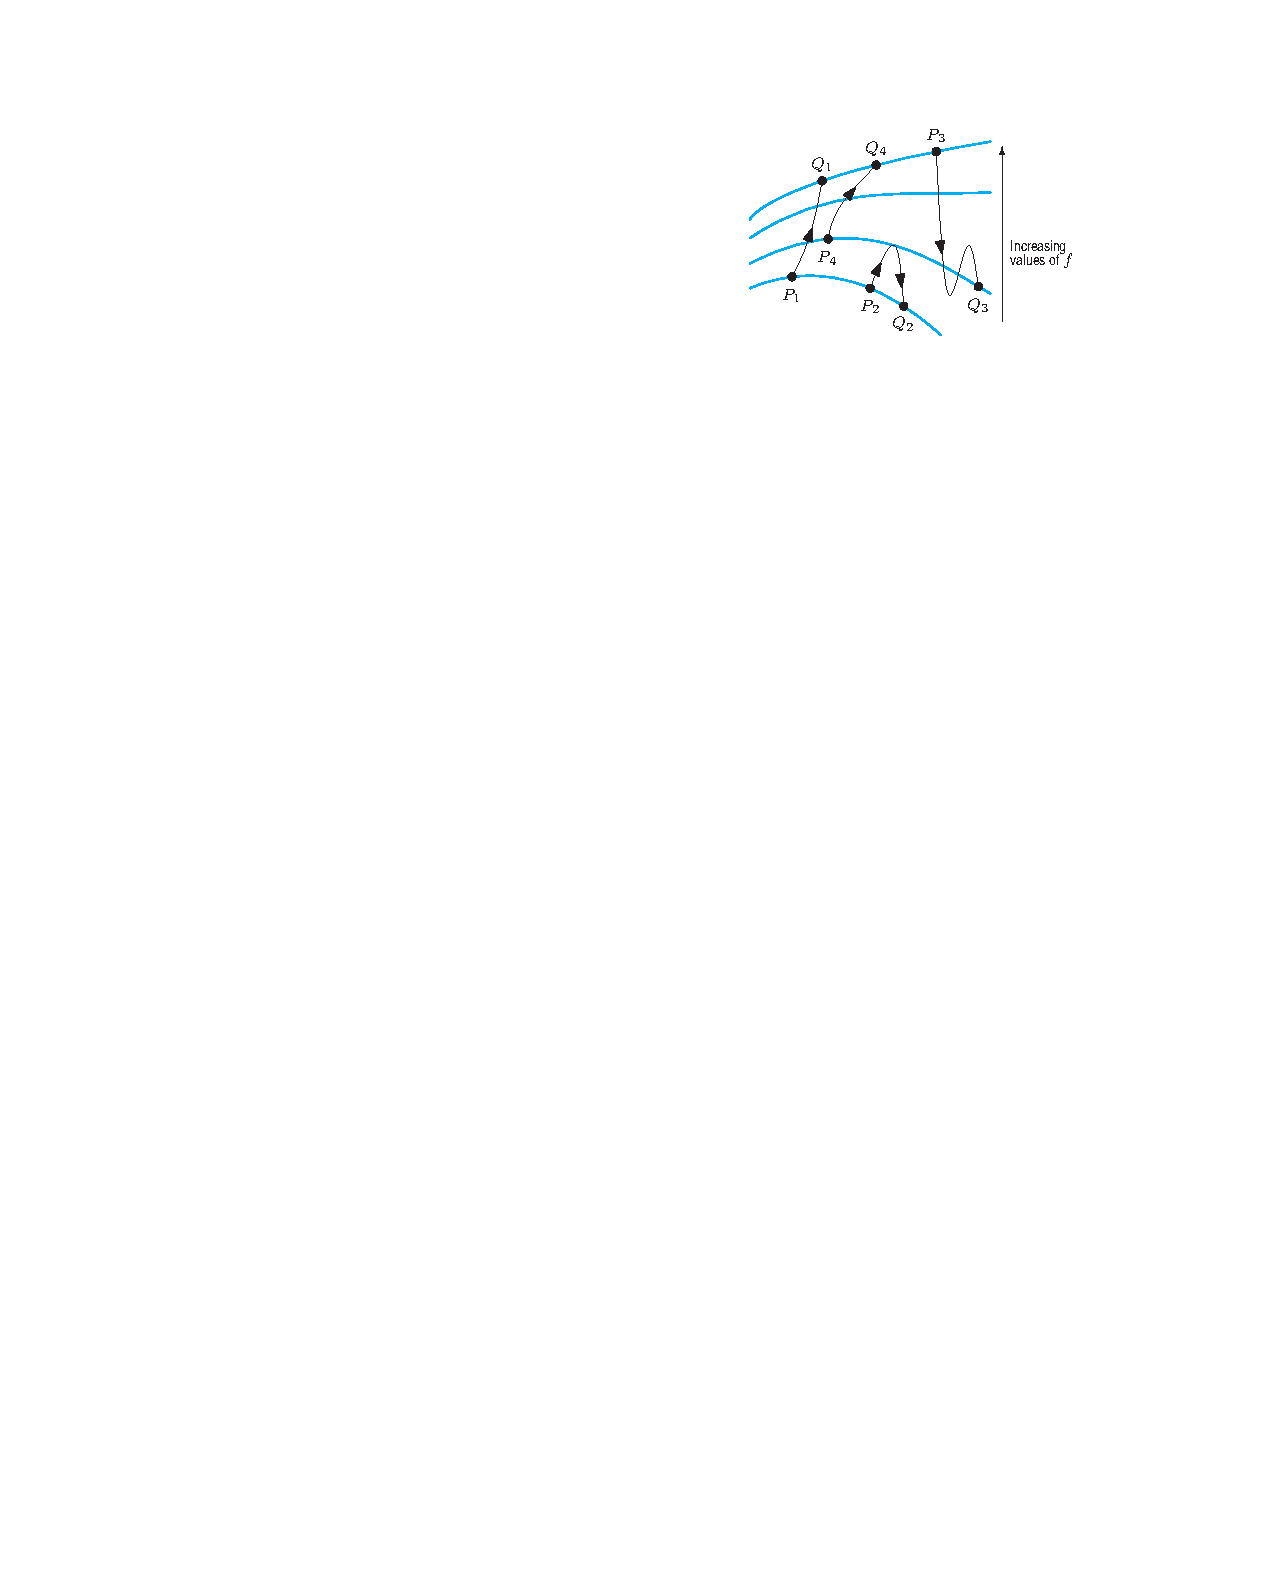
\includegraphics{img/HW09p1.pdf}

\begin{parts}
\item Which of the line integrals are zero, if any?
\begin{solution}
Using the fundamental theorem (which applies because $\vec F$ is a gradient field), $\int_C \vec F\cdot d\vec r = \int_C \nabla f\cdot d\vec r = f(\text{end})-f(\text{start})$.  The line integral will be zero when $f(\text{end}) = f(\text{start})$ which happens for curve $C_2$ (it starts and ends on the same contour).
\end{solution}
\item Arrange the line integrals in ascending order from least to greatest.
\begin{solution}
$f$ increases as we go upwards, so $C_3$ is connecting a start point at a higher $f$ to an end point at a lower $f$.  This one is negative.  $C_2$ results in a line integral of $0$.  The line integral for $C_4$ is positive and crosses just two contours while for $C_1$ it is positive and crosses three, so we have
\[\int_{C_3} \vec F\cdot d\vec r < \int_{C_2} \vec F\cdot d\vec r < \int_{C_4} \vec F\cdot d\vec r < \int_{C_1} \vec F\cdot d\vec r.\]
\end{solution}
\item Two of the line integrals have equal and opposite values.  Which are they?  Identify which is negative and which is positive.

\begin{solution}
We have $\int_{C_3} \vec F\cdot d\vec r$ as the only negative line integral, so it will have to be part of the ``equal and opposite''.  It crosses from the two contour to a contour two lower.  $\int_{C_4} \vec F\cdot d\vec r$ is a line integral between the same two contours, traversed in the opposite direction, so these are equal and opposite in value.  Note that they happen to be between the same two contours, but we can assume equal contour spacing, so this wasn't necessary.
\end{solution}

\end{parts}

% \question For the vector field $\displaystyle \frac{y}{x^2+y^2}\vec i - \frac{x}{x^2+y^2}\vec j$, \begin{parts}
% \item Show that it is irrotational.
% \begin{solution}
% We have $M = \frac{y}{x^2+y^2}$ and $N = \frac{-x}{x^2+y^2}$.

% $M_y = \frac{1}{x^2+y^2} + y(x^2+y^2)^{-2}(-1)(2y)$

% $N_x = \frac{-1}{x^2+y^2} - x(x^2+y^2)^{-2}(-1)(2x)$

% \[N_x - M_y = \frac{-1}{x^2+y^2} + (2x^2)(x^2+y^2)^{-2} - \frac{1}{x^2+y^2} + (2y^2)(x^2+y^2)^{-2}.\]

% Combining terms, we have

% \[N_x - M_y = \frac{-2}{x^2+y^2} + (2x^2+2y^2)(x^2+y^2)^{-2}.\]

% Simplifying:
% \[N_x - M_y = \frac{-2}{x^2+y^2} + (2)(x^2+y^2)^{-1} = 0.\]

% The vector field is irrotational.
% \end{solution}
% \item Identify a closed curve within the domain of $\vec F$ on which the circulation, $\oint_C \vec F\cdot d\vec r$, is nonzero.
% \begin{solution}
% The origin is missing from the domain so consider a path that encircles the origin.  Consider $x^2+y^2 = 1$ traversed counterclockwise.  We have $x=\cos t$ and $y = \sin t$.

% $\vec F(\cos t,\sin t) = \sin t \vec i - \cos t\vec j$ because $x^2 + y^2 = 1$ on this path.

% $\frac{d\vec r}{dt} = -\sin t \vec i + \cos t\vec j.$

% We have $\vec F\cdot \frac{d\vec r}{dt} = -\sin^2 t -\cos^2 t = -1$.

% \[\int_C \vec F \cdot d\vec r = \int_0^{2\pi} -1 \ dt = -2\pi.\]

% This is not zero, so there is a closed curve with nonzero circulation in this vector field.  It is irrotational but is not circulation free.
% \end{solution}
% \item Is the vector field a gradient field?  Justify your answer.
% \begin{solution}
% The vector field is not circulation free. Circulation free fields and gradient fields are equivalent, so it is not a gradient field.
% \end{solution}
% \end{parts}

\question An interesting device called a planimeter (\url{https://en.wikipedia.org/wiki/Planimeter}) returns an area when the operator traces the boundary of a shape.  The action of these devices is often explained via Green's theorem, with the ratchets in the device essentially doing a line integral.

\begin{parts}
\part Show that the line integral of the vector field $\vec F = x\vec j$ around any closed curve in the $xy$-plane, oriented as in Green's theorem, measures the area of the region enclosed by the curve.
\begin{solution}
We have $M = 0$ and $N=x$ so $N_x - M_y = 1$ for this vector field.  $C$ is a closed curve and is oriented so that Green's theorem applies.  Using Green's theorem, \[\int_C \vec F\cdot d\vec r = \int_R N_x - M_y dA = \int_R 1\ dA = \text{Area}(R),\]
so the line integral returns the area of the region enclosed!  This would be true any time $N_x - M_y = 1$.
\end{solution}

\item Provide a second vector field $\vec G$ with the same property (that $\displaystyle\oint_C \vec G\cdot d\vec r$ returns the area of the region enclosed by the curve).
\begin{solution}
Let $\vec G = -y\vec i$.  $N_x - M_y = -(-1) = 1$ so this vector field has the same property.
\end{solution}
\end{parts}

\end{questions}

\end{document}
